\documentclass{article}
\usepackage[utf8]{inputenc}
\usepackage[spanish]{babel}
\usepackage{subcaption}
\usepackage{graphicx}
\usepackage{pgffor}
\graphicspath{ {images/} }

\usepackage{color}
\definecolor{mygreen}{rgb}{0,0.6,0}
\definecolor{amber}{rgb}{1.0, 0.49, 0.0}

\usepackage{listings}
\lstdefinestyle{code}{
language=Octave,
frame=single,
breakatwhitespace=true,
breaklines=true,
basicstyle=\small\ttfamily,
tabsize=4,
numbers=left,
numberstyle=\tiny,
columns=fullflexible,
backgroundcolor=\color{white},
commentstyle=\color{mygreen},  % comment style
keywordstyle=\color{blue},     % keyword style
stringstyle=\color{amber},     % string literal style
}
\lstdefinestyle{snippet}{
language=Octave,
breakatwhitespace=true,
breaklines=true,
basicstyle=\small\ttfamily,
}
\lstdefinestyle{output}{
frame=single,
breakatwhitespace=true,
breaklines=true,
basicstyle=\small\ttfamily,
}

\addtolength{\textwidth}{1cm}
\addtolength{\textheight}{0.75cm}
\setcounter{section}{-1}

\title{Práctica 5}
\author{Héctor Laria Mantecón y Samuel Lapuente Jiménez}
\date{3 de diciembre de 2015}

\begin{document}

\maketitle

\section{Introducción}
El objetivo de la práctica es experimentar los efectos del sesgo y la varianza al trabajar con regresión logística.

\section{Regresión lineal regularizada}
Como podemos ver en la gráfica más abajo, el modelo es demasiado poco expresivo con un coeficiente, por lo que genera sesgo y produce un gran error aunque le demos más datos.

Esta es la función que calcula el coste y el gradiente.
\lstinputlisting[style=code]{src/linRCost.m}
Y en este script principal llamamos a esta función dentro de {\tt fmincg}.
\lstinputlisting[style=code]{src/uno.m}

Lo que nos da una gráfica de salida:
\begin{figure}[h]
\centering
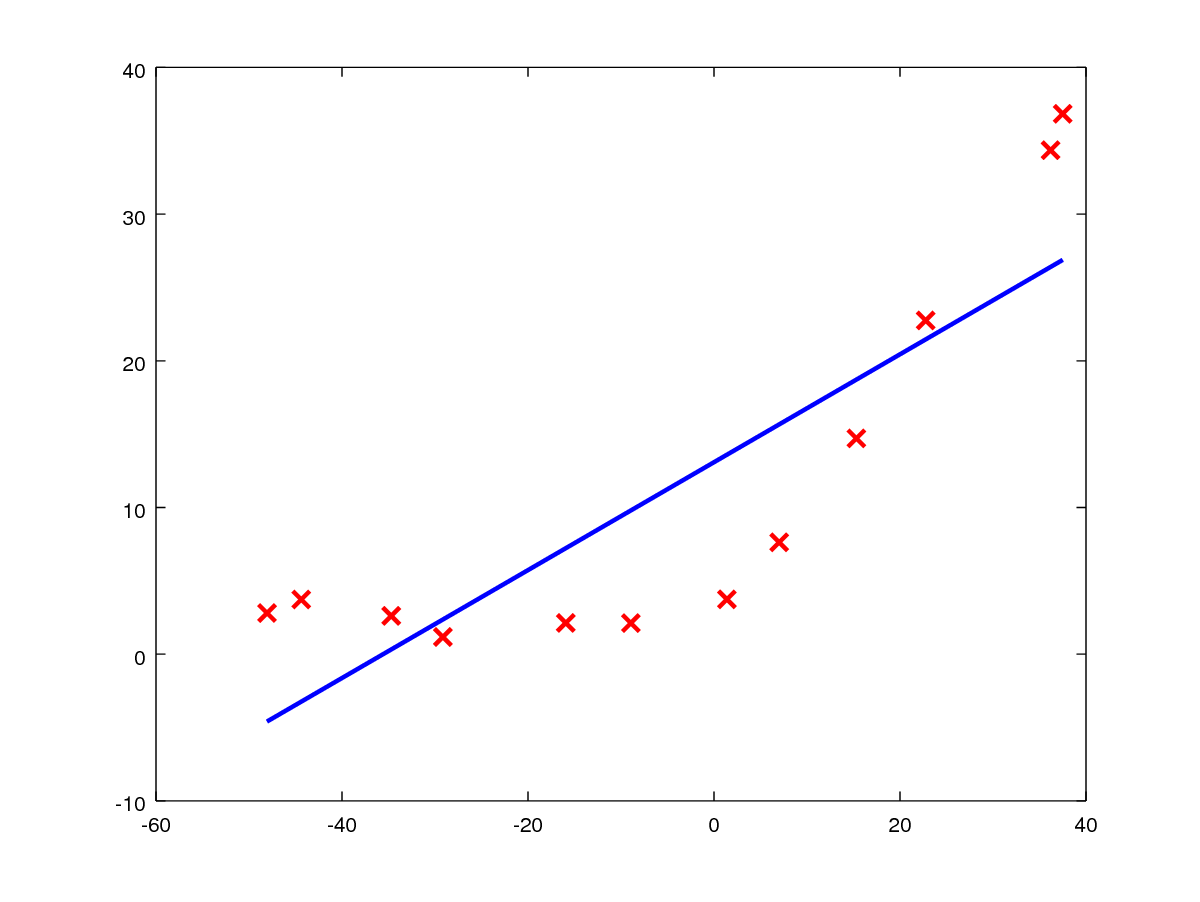
\includegraphics[width=\textwidth]{1}
\end{figure}

\pagebreak
\section{Curvas de aprendizaje}
Viendo la gráfica que se saca de calcular el error en los sucesivos subconjuntos de los casos de entrenamiento y validación, el error se estabiliza aunque añadamos más ejemplos de entrenamiento. Por lo que es notable que el modelo padece sesgo.

\begin{figure}[h]
\centering
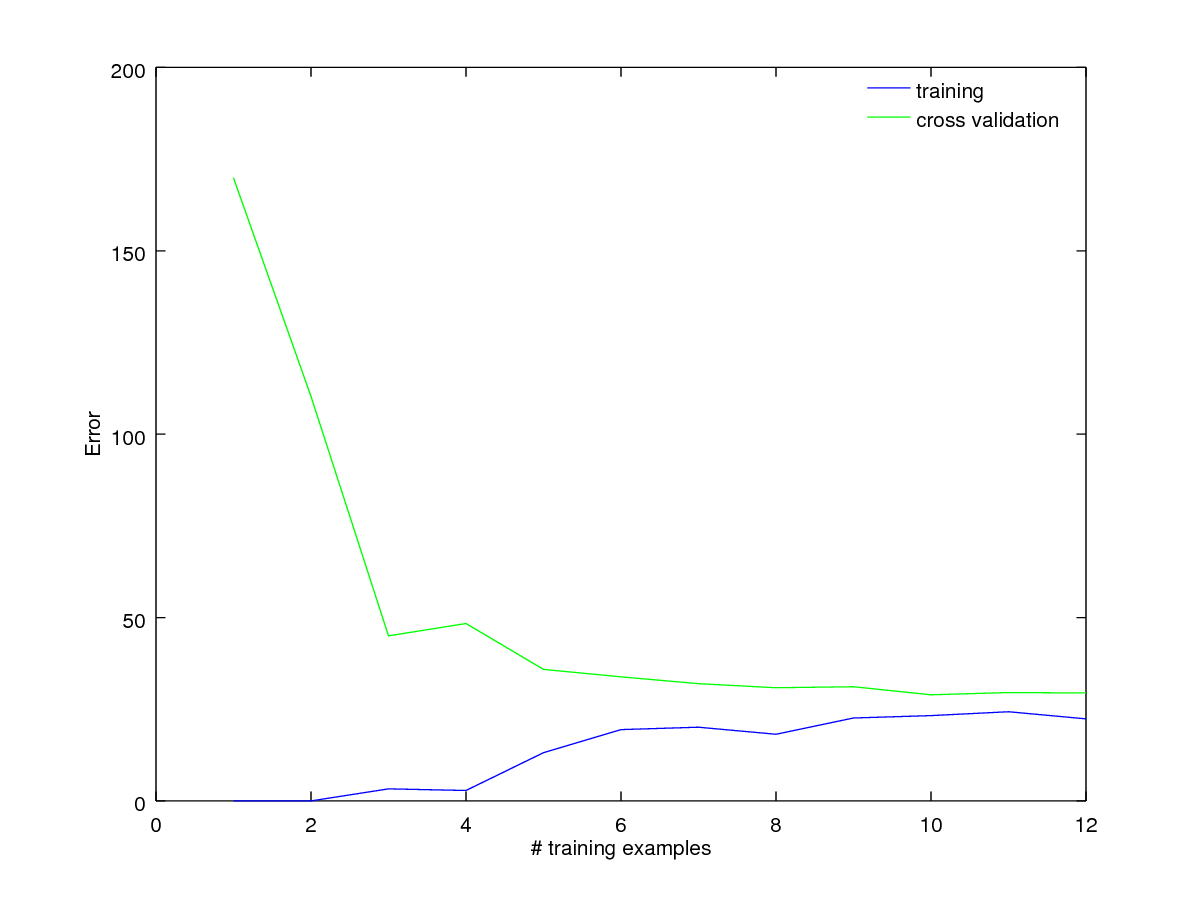
\includegraphics[width=\textwidth]{2}
\end{figure}

Para generar las curvas usamos el siguiente código:
\lstinputlisting[style=code]{src/dos.m}

\section{Regresión polinomial}
Cuantos más atributos tengamos más riesgo corremos de sobreajustarnos. Ademaś de tener que normalizarlos si hay mucha diferencia entre ellos (como de hecho hacemos con ayuda de {\tt featureNormalize}).
Podemos ver que con 8 atributos y una $\lambda$ muy pequeña el modelo efectivamente está sobreajustado.

\begin{figure}[h]
\centering
\includegraphics[width=\textwidth]{{{3.1}}}
\end{figure}

Como se ve en las gráficas sucesivas, con el cambio de $\lambda$ podemos arreglar esto.

La función que añade más atributos al modelo es la siguiente.
\lstinputlisting[style=code]{src/addFeatures.m}
Y este es el script principal de este apartado.
\lstinputlisting[style=code]{src/tres.m}

\begin{figure}
\vspace{-3cm}
{
\hspace{-3.8cm}
\begin{subfigure}{0.8\textwidth}
\includegraphics[width=\linewidth]{{{3.2.1}}}
\end{subfigure}
\hspace{-1cm}
\begin{subfigure}{0.8\textwidth}
\includegraphics[width=\linewidth]{{{3.2.2}}}
\end{subfigure}

\hspace{-3.8cm}
\begin{subfigure}{0.8\textwidth}
\includegraphics[width=\linewidth]{{{3.3.1}}}
\end{subfigure}
\hspace{-1cm}
\begin{subfigure}{0.8\textwidth}
\includegraphics[width=\linewidth]{{{3.3.2}}}
\end{subfigure}

\hspace{-3.8cm}
\begin{subfigure}{0.8\textwidth}
\includegraphics[width=\linewidth]{{{3.4.1}}}
\end{subfigure}
\hspace{-1cm}
\begin{subfigure}{0.8\textwidth}
\includegraphics[width=\linewidth]{{{3.4.2}}}
\end{subfigure}
}
\end{figure}

\pagebreak
\section{Selección del parámetro $\lambda$}
Para evitar caer en sesgo o sobreajuste comprobamos los resultados de diferentes modelos entrenados con diferentes $\lambda$. El código que produce eso es el siguiente.

\lstinputlisting[style=code]{src/cuatro.m}

En la salida del script podemos apreciar que el menor error será cuando $\lambda = 1$.

\begin{figure}[h]

\hspace{-3.8cm}
\begin{subfigure}{0.8\textwidth}
\includegraphics[width=\linewidth]{{{4.1}}}
\end{subfigure}
\hspace{-1cm}
\begin{subfigure}{0.8\textwidth}
\includegraphics[width=\linewidth]{{{4.2}}}
\end{subfigure}

\end{figure}

\section{Conclusión}
Como hemos podido comprobar en la práctica, un modelo con poca expresividad no puede ser refinado. Sin embargo uno con sobreajuste puede reducir su error al cambiar el coeficiente $\lambda$ (si no lo queremos cambiar podemos recurrir a usar más ejemplos de entrenamiento, entre otras).

Aunque hay que ser cuidadoso modificando $\lambda$ ya que puede pasar de un extremo a otro y llegar a tener sesgo. Un buen aliado son las curvas de aprendizaje siempre que tenemos que entrenar modelos.

\end{document}